\chapter*{Résumé en Français}
\addcontentsline{toc}{chapter}{Résumé en Français}%

% Neutron
Le neutron est une particule non élémentaire dépourvu de charge avec une masse proche de celle du proton. Il possède également un spin de $\frac{1}{2}$ et un moment magnétique faible. Le neutron étant une particule neutre, il n'interagit que très peu avec le cortège électronique du milieu contrairement aux particules chargées. Un neutron peut ainsi parcourir de grandes distances sans subir d’interactions majeures. Les interactions se faisant principalement avec les éléments du noyau par interaction forte. Les neutrons sont devenus des outils très intéressants pour de nombreux domaines de la science. Ces particules permettent de sonder la matière à différent niveau d'échelle et de temps via différentes méthodes. Les applications dépassent largement la physique et peuvent concerner des domaines variés comme la biologie, les sciences des matériaux et même l'archéologie.

% Sources neutrons
Cependant il est beaucoup plus compliqué de produire des neutrons que des particules chargées ou même des photons. Une des méthodes de production de neutrons consiste à utiliser des sources composites type alpha-béryllium. Cependant ces sources sont limitées à des faibles flux de neutrons. Les infrastructures de recherche actuelles reposent plutôt sur des réacteurs à fission. Un réacteur à fission produit un flux intense et continu de neutrons.
Le fonctionnement de ce type d’installation nécessite une gestion de la sécurité et des matières radioactives. Les réacteurs de recherche souffrent également de l’image du nucléaire ce qui peut freiner l’investissement dans ce type d’installation.

Depuis quelques années, les sources de neutrons pilotées par accélérateur sont devenues des alternatives crédibles face aux réacteurs et de nombreux projets de source à spallation ont vu le jour. Cela est rendu possible grâce aux progrès réalisés dans les technologies des accélérateurs de particules. Les sources se basant sur la spallation sont les plus efficaces mais aussi les plus complexes à mettre en oeuvre. Le fonctionnement de ce type de source est le suivant : des protons de hautes énergies (de la centaine de MeV au GeV) vont entrer en collision avec une cible dense. Les noyaux de la cible vont se désintégrer sous la violence du choc et des neutrons sont libérés sur un spectre très large. Les neutrons sont ensuite thermalisés et transportés vers différentes expériences. Les première sources à spallation ont vu le jours dans les années 70-80, puis une seconde génération a été developpée dans les années 2000. L'évolution des différentes sources de neutrons est montrée dans la Figure \ref{sumfr:fig:NeutronSources_a}.
\begin{figure}[!ht]
	\begin{subfigure}[t]{0.5\textwidth}
		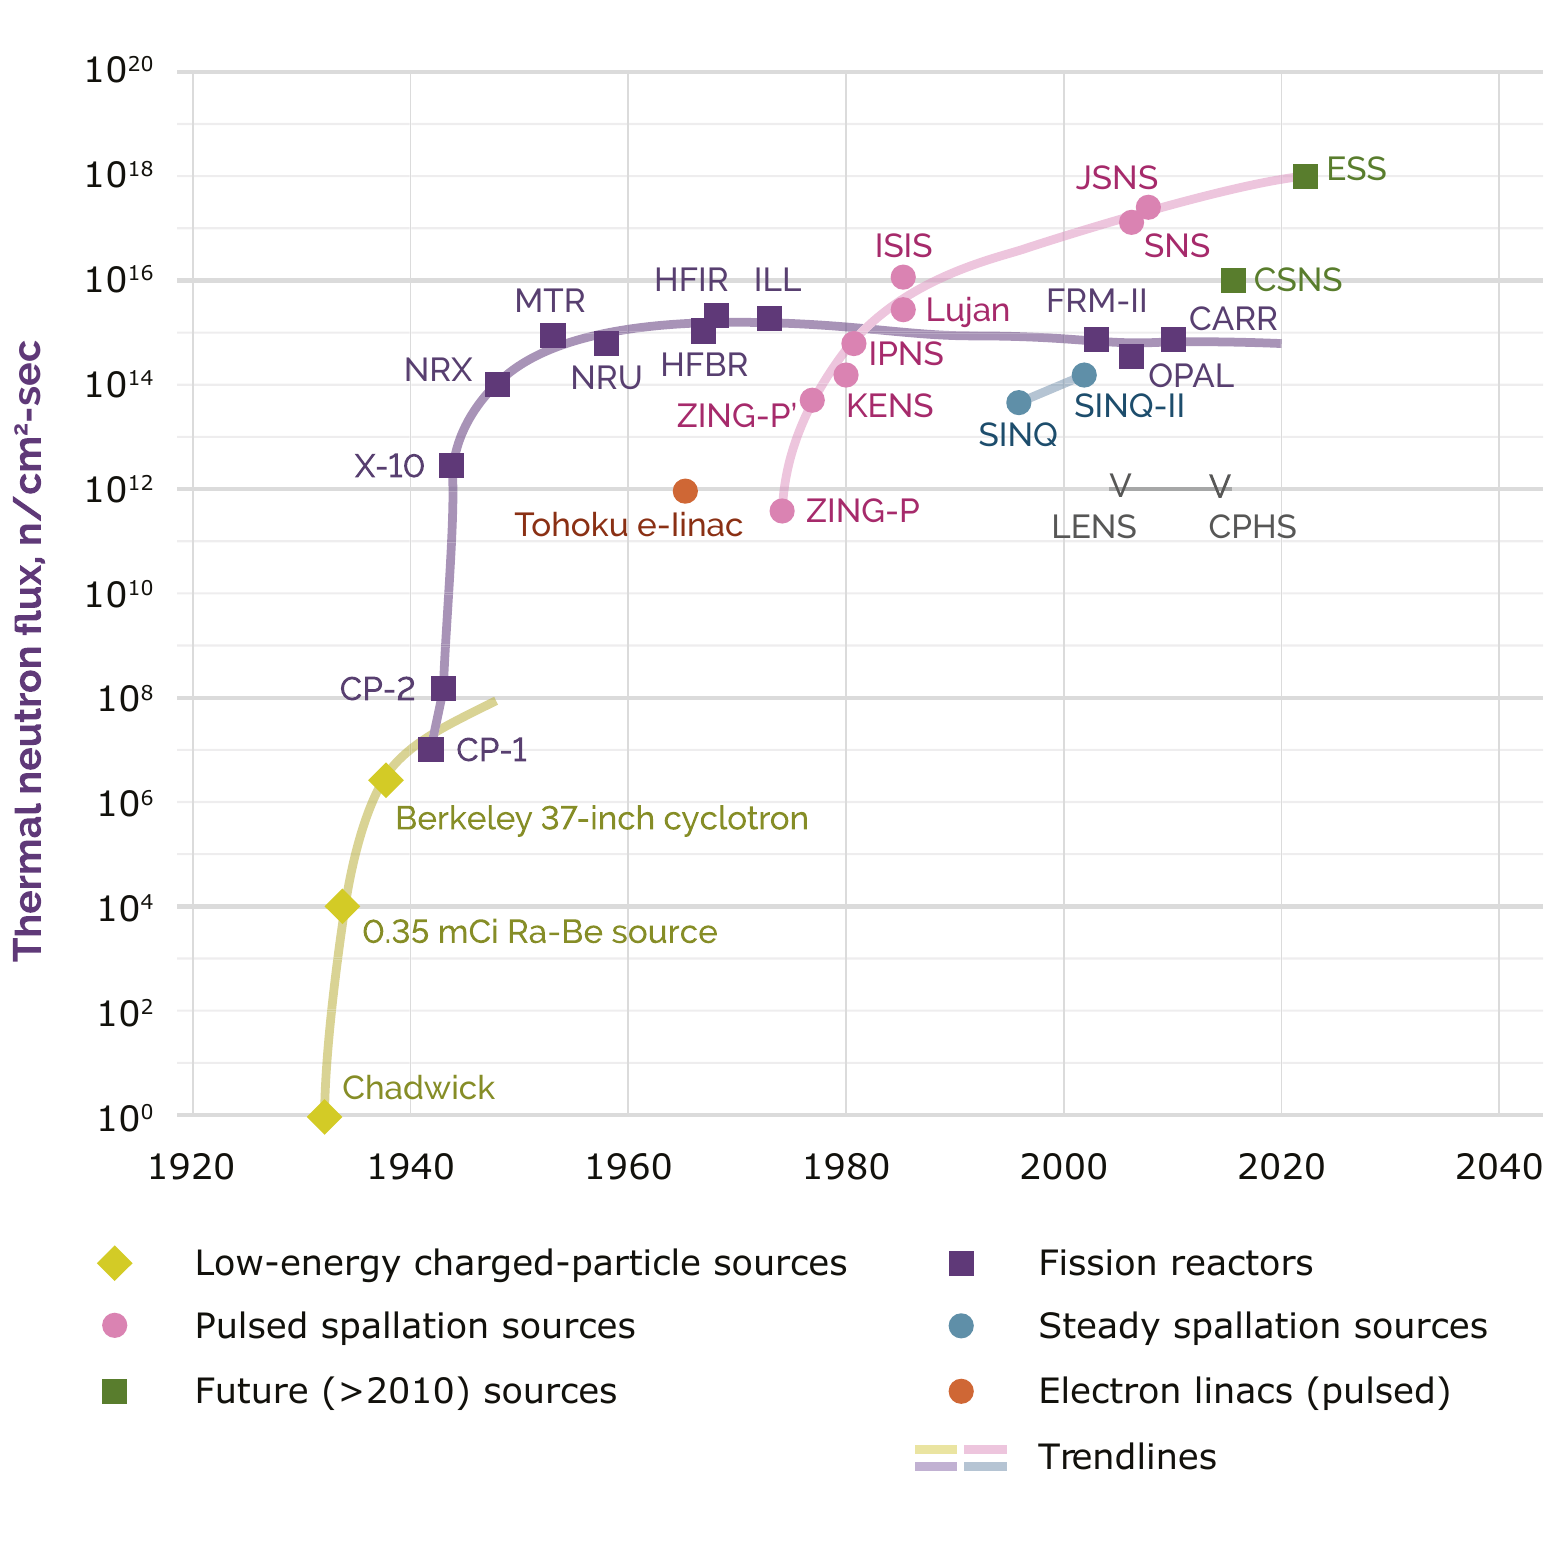
\includegraphics[width=\textwidth]{00_French/figures/fig000_NeutronSources_a}
		\caption[]{Evolution des sources de neutrons thermiques depuis la découverte du neutron.}
		\label{sumfr:fig:NeutronSources_a}
	\end{subfigure}
	~
	\begin{subfigure}[t]{0.5\textwidth}
		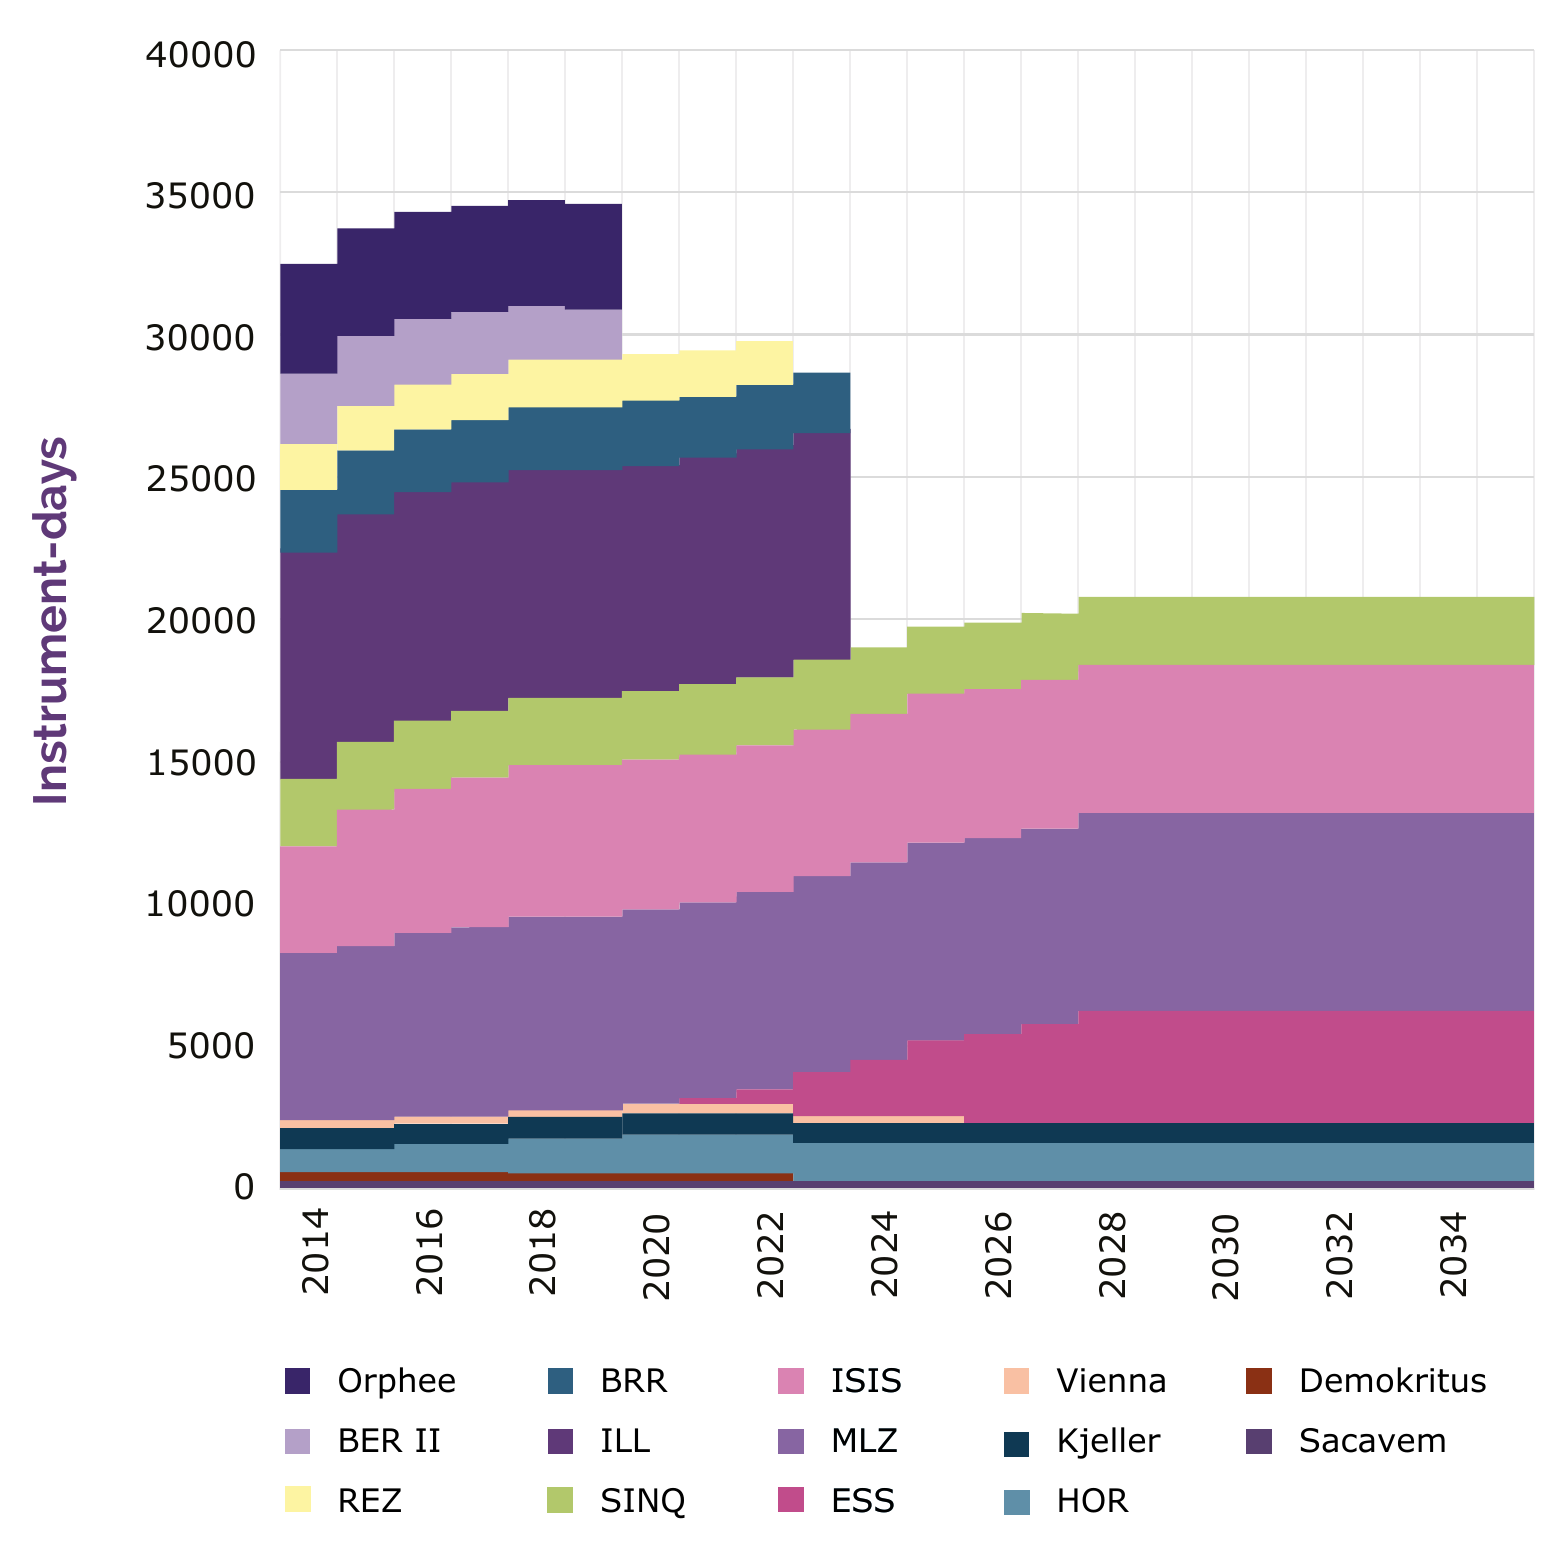
\includegraphics[width=\textwidth]{00_French/figures/fig000_NeutronSources_b}
		\caption[]{Prévision du temps instruments pour chaque source de neutrons Européennes.}
		\label{sumfr:fig:NeutronSources_b}
	\end{subfigure}
	\caption[]{Historique des sources de neutrons et prospectives Européennes  d'après un rapport de l'ESFRI datant de 2019.}
	\label{sumfr:fig:NeutronSources}
\end{figure}


Actuellement, les réacteurs de recherche sont les principales sources de neutrons en Europe. Cependant ces installations sont pour la plupart vieillissantes et aucune stratégie claire de renouvellement n'a été mise en oeuvre durant les dernières décennies. Ces installtions doivent fermer d'ici une dizaine d'années et l'accès aux sources de neutrons risque de devenir critique pour la  communauté scientifique Européenne, comme montré dans la Figure \ref{sumfr:fig:NeutronSources_b}. Pour conserver les compétences et les savoirs dans ces domaines, la communauté Européenne a impulsé un mouvement de renouveau se basant en partie sur la création d'une source de neutrons ultra intense nouvelle génération.

% ESS
La Source de Spallation Européenne (ESS) sera la future source à neutron, elle est actuellement en construction à Lund en Suède. L’objectif de ESS est de devenir la source de neutron pulsée la plus brillante au monde. La Figure \ref{sumfr:fig:ESS_pulse} montre les différences en terme de brillance entre ESS et les sources existantes. Les premiers neutrons sont attendus pour 2022 afin de prévenir la fermeture des principaux réacteurs  d’ici les prochaines années. Lors du démarrage du faisceau, 15 instruments de spectroscopie, de réflectométrie et de diffraction neutronique seront disponibles pour les chercheurs et les partenaires industriels dans des domaines variés. Puis dans une phase d’extension, 7 nouveaux instruments seront installés à ESS.
\begin{figure}[!ht]
  \begin{center}
    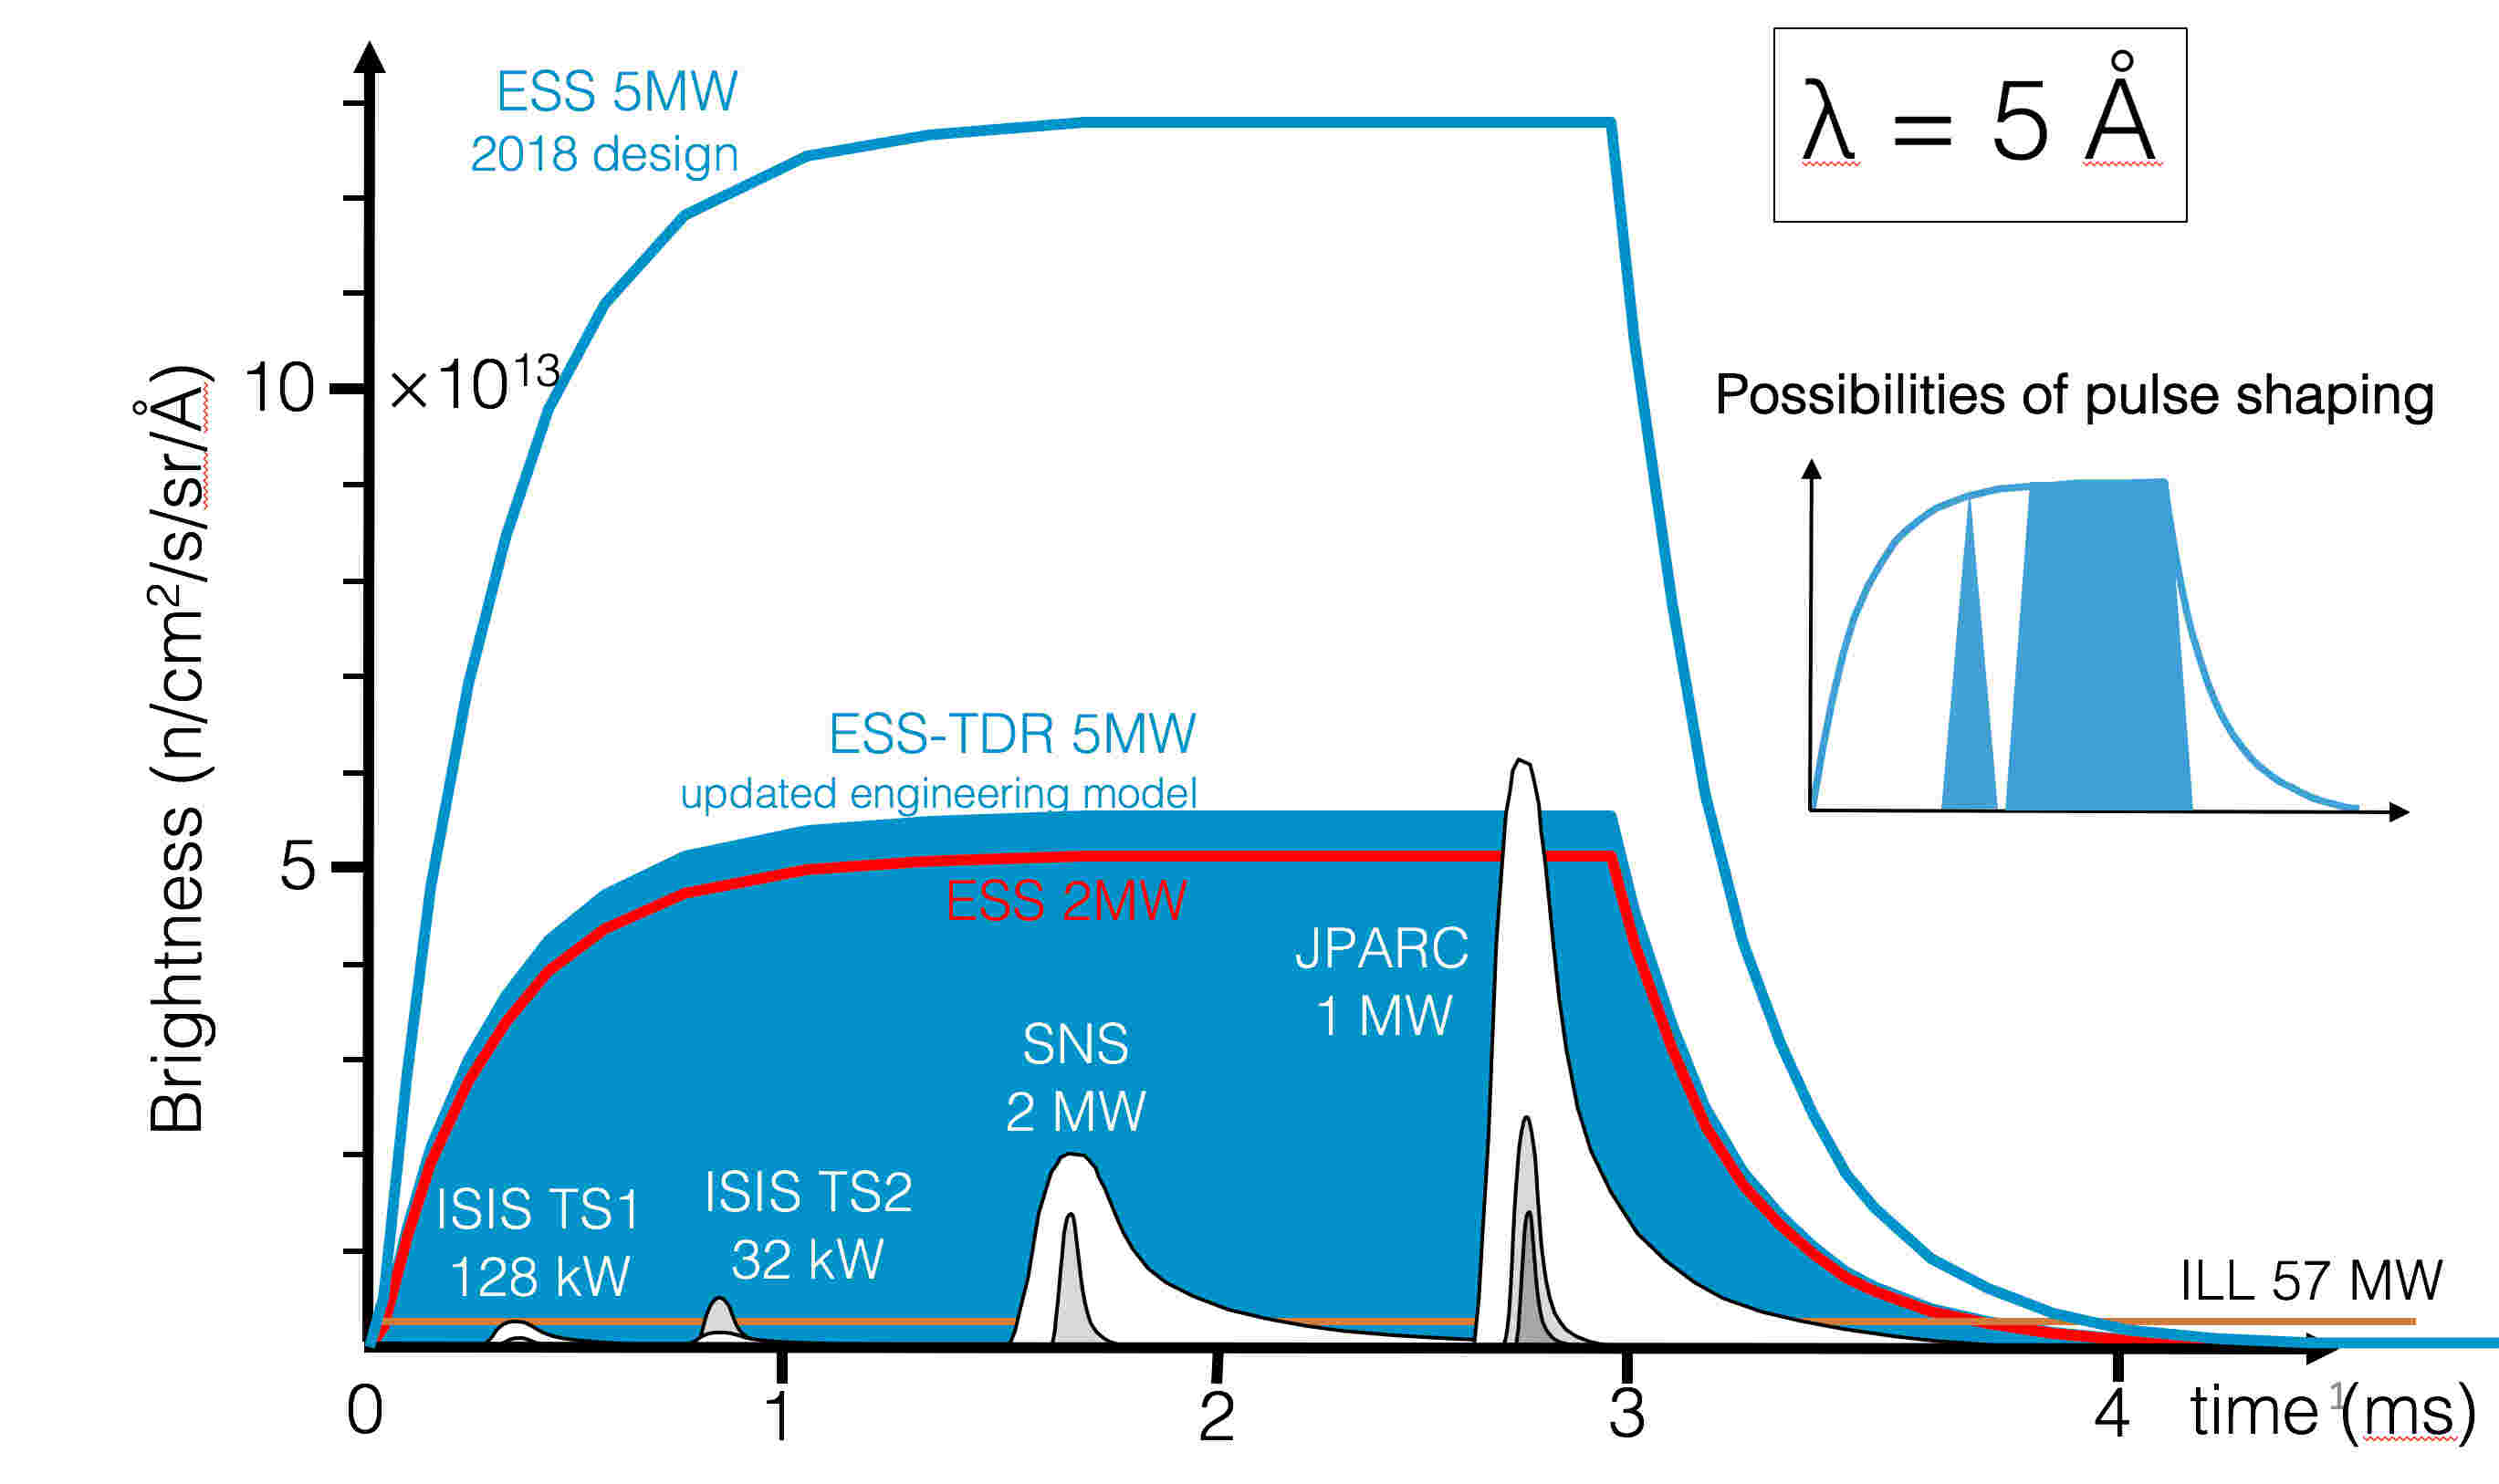
\includegraphics[width=0.85\textwidth]{00_French/figures/fig000_ESS_pulse}
  \end{center}
  \caption[]{Comparaison de la brillance d'ESS par rapport aux différentes sources de neutrons existantes.}
  \label{sumfr:fig:ESS_pulse}
\end{figure}


ESS peut être résumée grossièrement en 3 parties : un puissant accélérateur linéaire (linac), une imposante cible en tungstène et une dizaine d’instruments à neutrons. Chacun de ces éléments représente une rupture technologique dans leur domaine respectif. La spécificité de ESS est son accélérateur linéaire de haute intensité qui sera l’un des accélérateurs pulsé les plus puissant au monde. Pour se faire, l’accélérateur de ESS se base massivement sur des cavités supraconductrices qui permettent d'accélérer des impulsions longues et intenses dans des dimensions raisonnables. Le coût total de construction est estimé à $1$ milliard € et le coût de fonctionnement annuel sera d'environ $100$ million €.
\begin{figure}[!ht]
	\begin{center}
		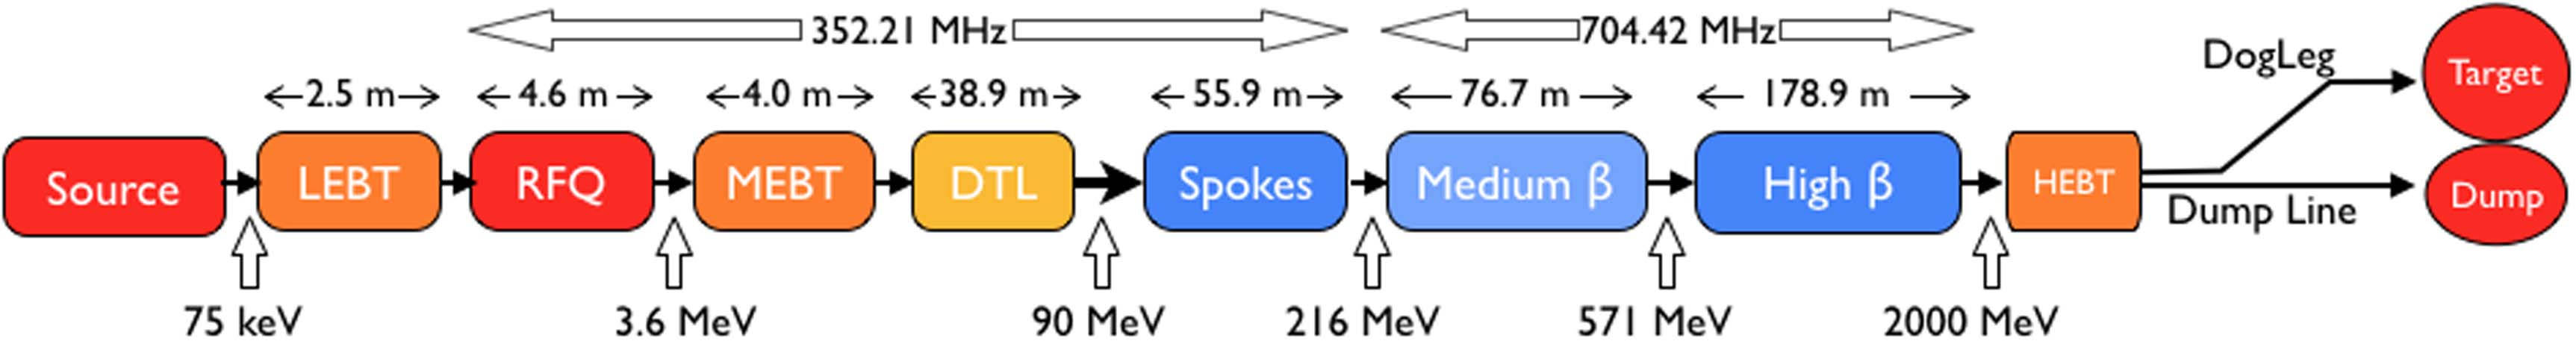
\includegraphics[width=\textwidth]{00_French/figures/fig000_ESS_acc}
	\end{center}
	\caption[]{Représentation simplifiée du linac de ESS. Les blocs bleus représentent la partie supraconductrice de l'accélérateur où les IPM seront installés.}
	\label{sumfr:fig:ESS_acc}
\end{figure}


% IPM
Les diagnostics faisceau servent à s’assurer du bon fonctionnement de l'accélérateur et garantissent la sécurité des personnes et des installation en cas de dysfonctionnement. Ils permettent de mesurer différentes caractéristique du faisceau comme le courant, la position, l’énergie, les pertes. Pour chaque caractéristiques du faisceau plusieurs méthodes peuvent être considérées avec pour chacune des avantages et des inconvénients. Les diagnostic faisceau sont donc à la croisée de nombreux domaines de la physique.

La mesure de profile transverse donne une information sur la répartition du faisceau dans le plan transverse. C'est une donnée très intéressante pour les physiciens de la dynamique faisceau. Les mesures de profil transverse peuvent être séparées en deux types. Les méthodes intrusives ou invasives qui entrent en interaction directe avec le faisceau allant même jusqu'à le détruire. Et les méthodes non invasives qui ont des interactions négligeables ou nulles avec le faisceau. Dans la partie supraconductrice de ESS, la mesure du profil dans les conditions nominales doit se faire de manière non invasive. La méthode retenue est basée sur la collection directe des produits d'ionisation du gaz résiduel par un champ électrique. Ce type de moniteurs est appelé Ionization Profile Monitor (IPM). Son principe de fonctionnement est illustré dans la Figure \ref{sumfr:fig:ipm_outline} et peut être synthétisé en trois grandes étapes:
\begin{wrapfigure}{r}{0.5\textwidth}
	\centering
	\begin{tikzpicture}%[scale=1.3]
		% Variables
		% Ipm
		\pgfmathsetmacro{\LIPM}{1.8};
		\pgfmathsetmacro{\HIPM}{1.8};
		\pgfmathsetmacro{\TIPM}{0.1};
		% Deg
		\pgfmathsetmacro{\LDEG}{0.1};
		\pgfmathsetmacro{\HDEG}{0.3};
		\pgfmathsetmacro{\NDEG}{6};
		\pgfmathsetmacro{\SDEG}{1.5};
		\pgfmathsetmacro{\SPAND}{(2*\SDEG - \HDEG)/\NDEG}

		\draw[] (\LIPM,0) node[right,align=left] {Field\\correctors\\or\\degraders};

		% Beam
		\draw[fill=blue!30] (0,0) circle (0.4) node[left,xshift = -0.3cm] {Faisceau};
		% Cage
		\draw (0,0) (-\LIPM,\HIPM)rectangle(\LIPM,\HIPM+\TIPM) node[above] {Anode};
		\draw (0,0) (-\LIPM,-\HIPM)rectangle(\LIPM,-\HIPM-\TIPM) node[below] {Cathode};
		\draw[fill=red!50] (-\LIPM/2,-\HIPM) rectangle(\LIPM/2,-\HIPM-\TIPM) node[midway,below] {Détecteur};
		% Ionized particle
		\draw[blue, dashed,->] (0.1,0.8)--(0.1,\LIPM);
		\draw[blue,fill=blue] (0.1,0.8) circle [radius=1mm] node[] {\tiny\color{white}{$-$}};

		\draw[red, dashed,->] (0.16,-1)--(0.16,-\LIPM);
		\draw[red,fill=red] (0.16,-1) circle [radius=1mm] node[] {\tiny\color{white}{$+$}};

		\draw[blue,dashed,->] (-0.1,0.1)--(-0.1,\LIPM);
		\draw[blue,fill=blue] (-0.1,0.1) circle [radius=1mm] node[] {\tiny\color{white}{$-$}};

		\draw[red,dashed,->] (-0.1,-0.1)--(-0.1,-\LIPM);
		\draw[red,fill=red] (-0.1,-0.1) circle [radius=1mm] node[] {\tiny\color{white}{$+$}};

		%Field
		\draw[->] (-1.2,1.5)--(-1.2,0.6) node [midway,right]{$\vec{E}$};
		% Degradors
		\foreach \x in {0,...,\NDEG}{
				\draw (0,0) (-\LIPM,\x*\SPAND - \SDEG) rectangle (-\LIPM+\LDEG,\x*\SPAND+\HDEG-\SDEG);
				\draw (0,0) (\LIPM,\x*\SPAND - \SDEG) rectangle (\LIPM-\LDEG,\x*\SPAND+ \HDEG-\SDEG);}


		%Profile
		\begin{axis}[every axis plot post/.append style={
						mark=none,domain=-3:3,samples=50,smooth},
				clip=false,
				axis y line=none,
				axis x line*=bottom,
				ymin=0,
				ymax=1,
				xtick=\empty,
				width=4cm,
				height=3cm,
				scale only axis,
				xshift=-2cm,
				yshift=-3.5cm
			]
			\addplot {\gauss{0}{0.3}{0.3}};
		\end{axis}

	\end{tikzpicture}
	\centering
	\caption[]{Représentation synthétique du fonctionnement d'un IPM}
	\label{sumfr:fig:ipm_outline}
\end{wrapfigure}

\begin{enumerate}
  \item Les protons du faisceau passent à travers le gas résiduel dans la chambre de d'accélérateur. Cela induit une ionization: des paires électron/ion sont créées.
  \item Dans l'IPM, un fort champ électrique conduit les électrons ou les ions\footnote{Cela dépend de la polarisation de l'IPM.} vers un système de détection segmenté.
  \item Le profil est reconstruit dans une direction transverse. Pour un profil complet, une paire d'IPM, avec un IPM tourné de $90\textdegree{}$ par rapport à l'autre, est nécessaire.
\end{enumerate}
Les IPM sont assez communs sur les anneaux de stockage de protons/hadrons où les pressions sont très basses. L’utilisation de plus en plus fréquente des cavités supraconductrices dans les accélérateurs linéaires fait que cette méthode devient également intéressante pour ce type d'accélérateurs. Cette thèse présente le travail effectué lors du développement d’un IPM pour la partie supraconductrice de l’accélérateur de ESS.

% Simulation
La simulation d’un IPM est décomposée de la même façon que son fonctionnement décrit plus haut. Dans un premier temps il convient de savoir si le nombre de particules initialement créées est suffisant pour être détecté. Cependant ce nombre de particules ne donne pas la certitude de pouvoir mesurer un profil correct. Il faut prendre en compte les différents effets électromagnétiques qui vont influer sur la trajectoire des particules. Ces effets peuvent changer la projection du profil et faire perdre des particules. La dernière étapes consiste à évaluer la réponse de l'élément de détection en fonction des caractéristiques de la particule incident. La nature du détecteur change aussi profondément la modélisation de la réponse.

% TODO: Finir
Lorsque les protons du faisceau passent dans le gaz résiduel ils vont générer un certain nombre de paires électron/ion. Ce nombre dépends fortement des caractéristiques des protons (énergies, nombres) mais aussi celles du milieu (composition, densité). Il est primordial de savoir si ce nombre est suffisant pour permettre une mesure correcte. C'est pourquoi l'estimation du nombre de produits d'ionisation a été réalisée à partir de deux méthodes :
\begin{itemize}
  \item Calculs directs à partir du modèle de Bethe.
  \item Simulation en utilisant les codes Garfield++/Heed++.
\end{itemize}
La Table \ref{sumfr:table:GarfieldBethe} récapitule les résultats des différentes méthodes de calcul. Le signal primaire attendu est de l'ordre de quelques dizaines de milliers de particules par impulsion de faisceau. Le système de détection doit être suffisamment sensible à ces niveaux.
\begin{table}[ht]%{r}{0.5\textwidth}
	\centering
	\caption[]
	{Comparaison entre le nombre d'électrons d'ionisation par calcul direct de l'équation de Bethe et par des simulations Garfield++/Head++.}
	\label{sumfr:table:GarfieldBethe}
	\begin{tabularx}{\linewidth}{XXXX}
		\toprule
		Energie    & \(N_{Bethe}\) & \(N_{garfield}\) & Facteur \\
		\midrule
		\(97.2\)  & \(100210\)    & \(52500\)             & \(0.52\)   \\
		\(231.4\) & \(54970\)     & \(27500\)             & \(0.50\)   \\
		\(278.9\) & \(49160\)     & \(26100\)             & \(0.53\)   \\
		\(315.8\) & \(45850\)     & \(23800\)             & \(0.52\)   \\
		\(628.3\) & \(33600\)     & \(17500\)             & \(0.52\)   \\
		\bottomrule
	\end{tabularx}
\end{table}

Mais avant de choisir le système de détection, il convient d'étudier la trajectoire des particules dans l'IPM.
Un IPM peut être vu comme un détecteur à plaques parallèles. Dans un IPM idéal, ces plaques sont infinies. Dans la réalité, les plaques ne peuvent être considérées comme infinies car la distance entre les deux électrodes est égale à la taille de l'IPM. Dans ces conditions le champ n’est plus du tout uniforme dans l'IPM. Des simulations COMSOL ont été effectuées afin de quantifier ces effets et les corriger à l'aide de correcteurs de champ. La Figure \ref{sumfr:fig:Field} montre l'importance des correcteurs pour obtenir une mesure correcte du profil.
\begin{figure}[!ht]
	\begin{subfigure}[t]{0.5\textwidth}
		\includesvg[width=\textwidth]{00_French/figures/fig000_Field_a}
		\caption[]{Simulations d'une mesure de profil sans correction des non uniformités.}
		\label{sumfr:fig:Field_a}
	\end{subfigure}
	~
	\begin{subfigure}[t]{0.5\textwidth}
		\includesvg[width=\textwidth]{00_French/figures/fig000_Field_b}
		\caption[]{Simulations d'une mesure de profil avec correction des non uniformités.}
		\label{sumfr:fig:Field_b}
	\end{subfigure}
  \caption[]{Simulations d'une mesure de profil en considérant les non uniformités au sein de l'IPM. Les corrections sont obligatoires pour mesurer correctement le profil.}
	\label{sumfr:fig:Field}
\end{figure}


\begin{wrapfigure}{r}{0.65\textwidth}  
  \includesvg[width=0.65\textwidth]{00_French/figures/fig000_SC2_fr}
  \caption[]{Simulations d'un mesure de profil en considérant la charge d'espace pour les ions et les électrons.}
  \label{sumfr:fig:SC2_fr}
\end{wrapfigure}

Un autre effet qui peut grandement affecter la trajectoire des particules est la charge d'espace. Dans le référentiel de l'IPM les protons d'un bunch faisceau sont en mouvement il y a donc création d’un fort champ électrique radial et d'un champ magnétique autour de l'axe faisceau. Des simulations, dont un exemple est donné dans la Figure \ref{sumfr:fig:SC2_profile}, ont montré clairement que les ions sont moins sensibles au phénomène de charge d’espace et de vitesse initiale. 
La mesure avec des électrons introduit une erreur qui ne permet pas de satisfaire les prérequis d’ESS. Il est impossible d’installer un aimant correcteur pour contraindre les trajectoires des électrons. Par conséquent la mesure du profil s’effectuera en ions.

Les caractéristiques (énergies, trajectoires) des particules à détecter sont connues. Il faut maintenant étudier le système qui va les détecter. Trois systèmes ont été selectionnés avec chacun des avantages et des inconvénients:
\begin{itemize}
  \item Un plancher de pistes conductrices qui est une méthode simple et robuste mais peu sensible car dépourvue d'étage d'amplification. Les performances dépendent de l'électronique de lecture qui est complexe.
  \item Une galette micro canaux  (MCP), qui est un amplificateur à électrons. Elle est ensuite couplée à un plancher de pistes ou un écran phosphorescent. Dans ce dernier cas, l'électronique de lecture est simple: une caméra. Un MCP a l'inconvénient de se détériorer au fur et à mesure.
  \item Un détecteur silicium semi-conducteur qui a une bonne sensibilité et des performances élevées. Cependant la détection n'est pas assurée si les ions sont utilisés.
\end{itemize}
Les résultats des différentes simulations ont été exposés lors d'une Preliminary Design Review comportant un Go/NoGo passé avec succès. Dès lors le travail c'est concentré sur la réalisation de prototypes.

% Test
Les nombreuses simulations nous ont permis de converger sur un design d’IPM qui pourrait fonctionner avec les conditions ESS. Cependant, les simulations n'éclaircissent pas tous les points critiques du projet et en particulier sur la problématique des systèmes de détection. Pour toutes ces raisons et au vu de la criticité du projet la construction, des tests de prototypes s’imposent. La construction et les tests de prototypes est aussi un formidable moyen d'obtenir une expérience et un retour d'expérience avant la phase de production des détecteurs finaux.

% IRMA
\begin{figure}[!ht]
  \centering
  \begin{subfigure}[t]{0.275\textwidth}
    \includesvg[width=\textwidth]{00_French/figures/fig000_IRMA_12keV_fr}
    \caption[]{Signal à $12\,\mathrm{keV}$.}
    \label{sumfr:fig:IRMA_a}
  \end{subfigure}
  ~
  \begin{subfigure}[t]{0.275\textwidth}
    \includesvg[width=\textwidth]{00_French/figures/fig000_IRMA_15keV_fr}
    \caption[]{Signal à $15\,\mathrm{keV}$.}
    \label{sumfr:fig:IRMA_b}
  \end{subfigure}
  ~
  \begin{subfigure}[t]{0.33\textwidth}
    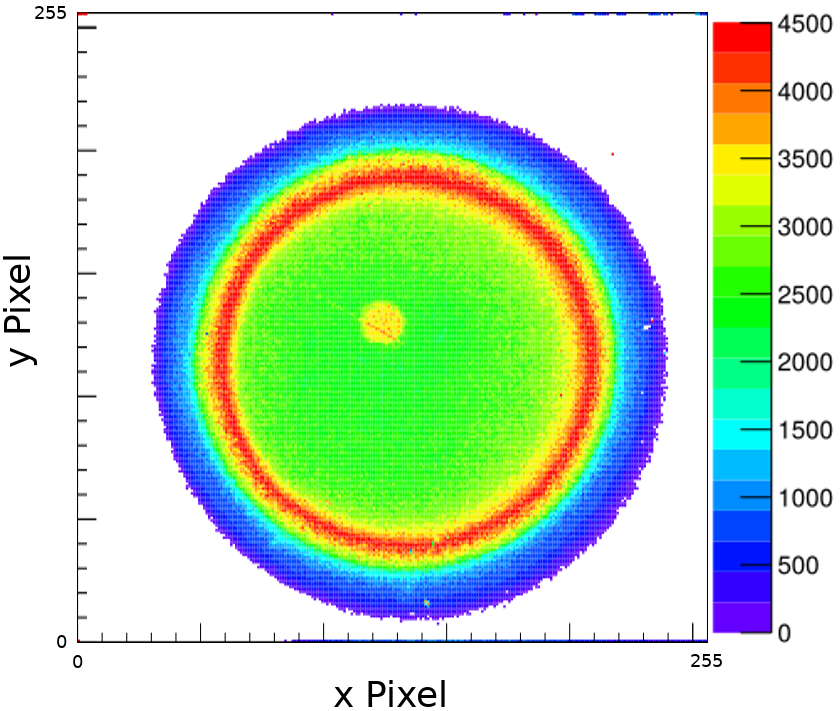
\includegraphics[width=\textwidth]{00_French/figures/fig000_IRMA_damage3_fr}
    \caption[]{La zone est endommagée après l'irradiation.}
    \label{sumfr:fig:IRMA_c}
  \end{subfigure}
  \caption[]{Résultats des tests effectués sur le détecteur $Si$ à l'aide d'un implanteur d'ions.}
  \label{sumfr:fig:IRMA}
\end{figure}
Dans un premier temps nous avons essayé de déterminer si les détecteur silicium pouvaient fonctionner en mode détection d’ions. A l’aide de l’équipe du CERN qui utilise ce type détecteur, nous avons pu tester un détecteur silicium avec un implanteur d’ions. Les premiers résultats montrent que la mesure est possible mais ne laisse pas de marge d'erreur ainsi qu'une possible déterioration du capteur. Ce système de détection a été écarté pour la version finale des IPM.

% TB
\begin{wrapfigure}{r}{0.35\textwidth}  
  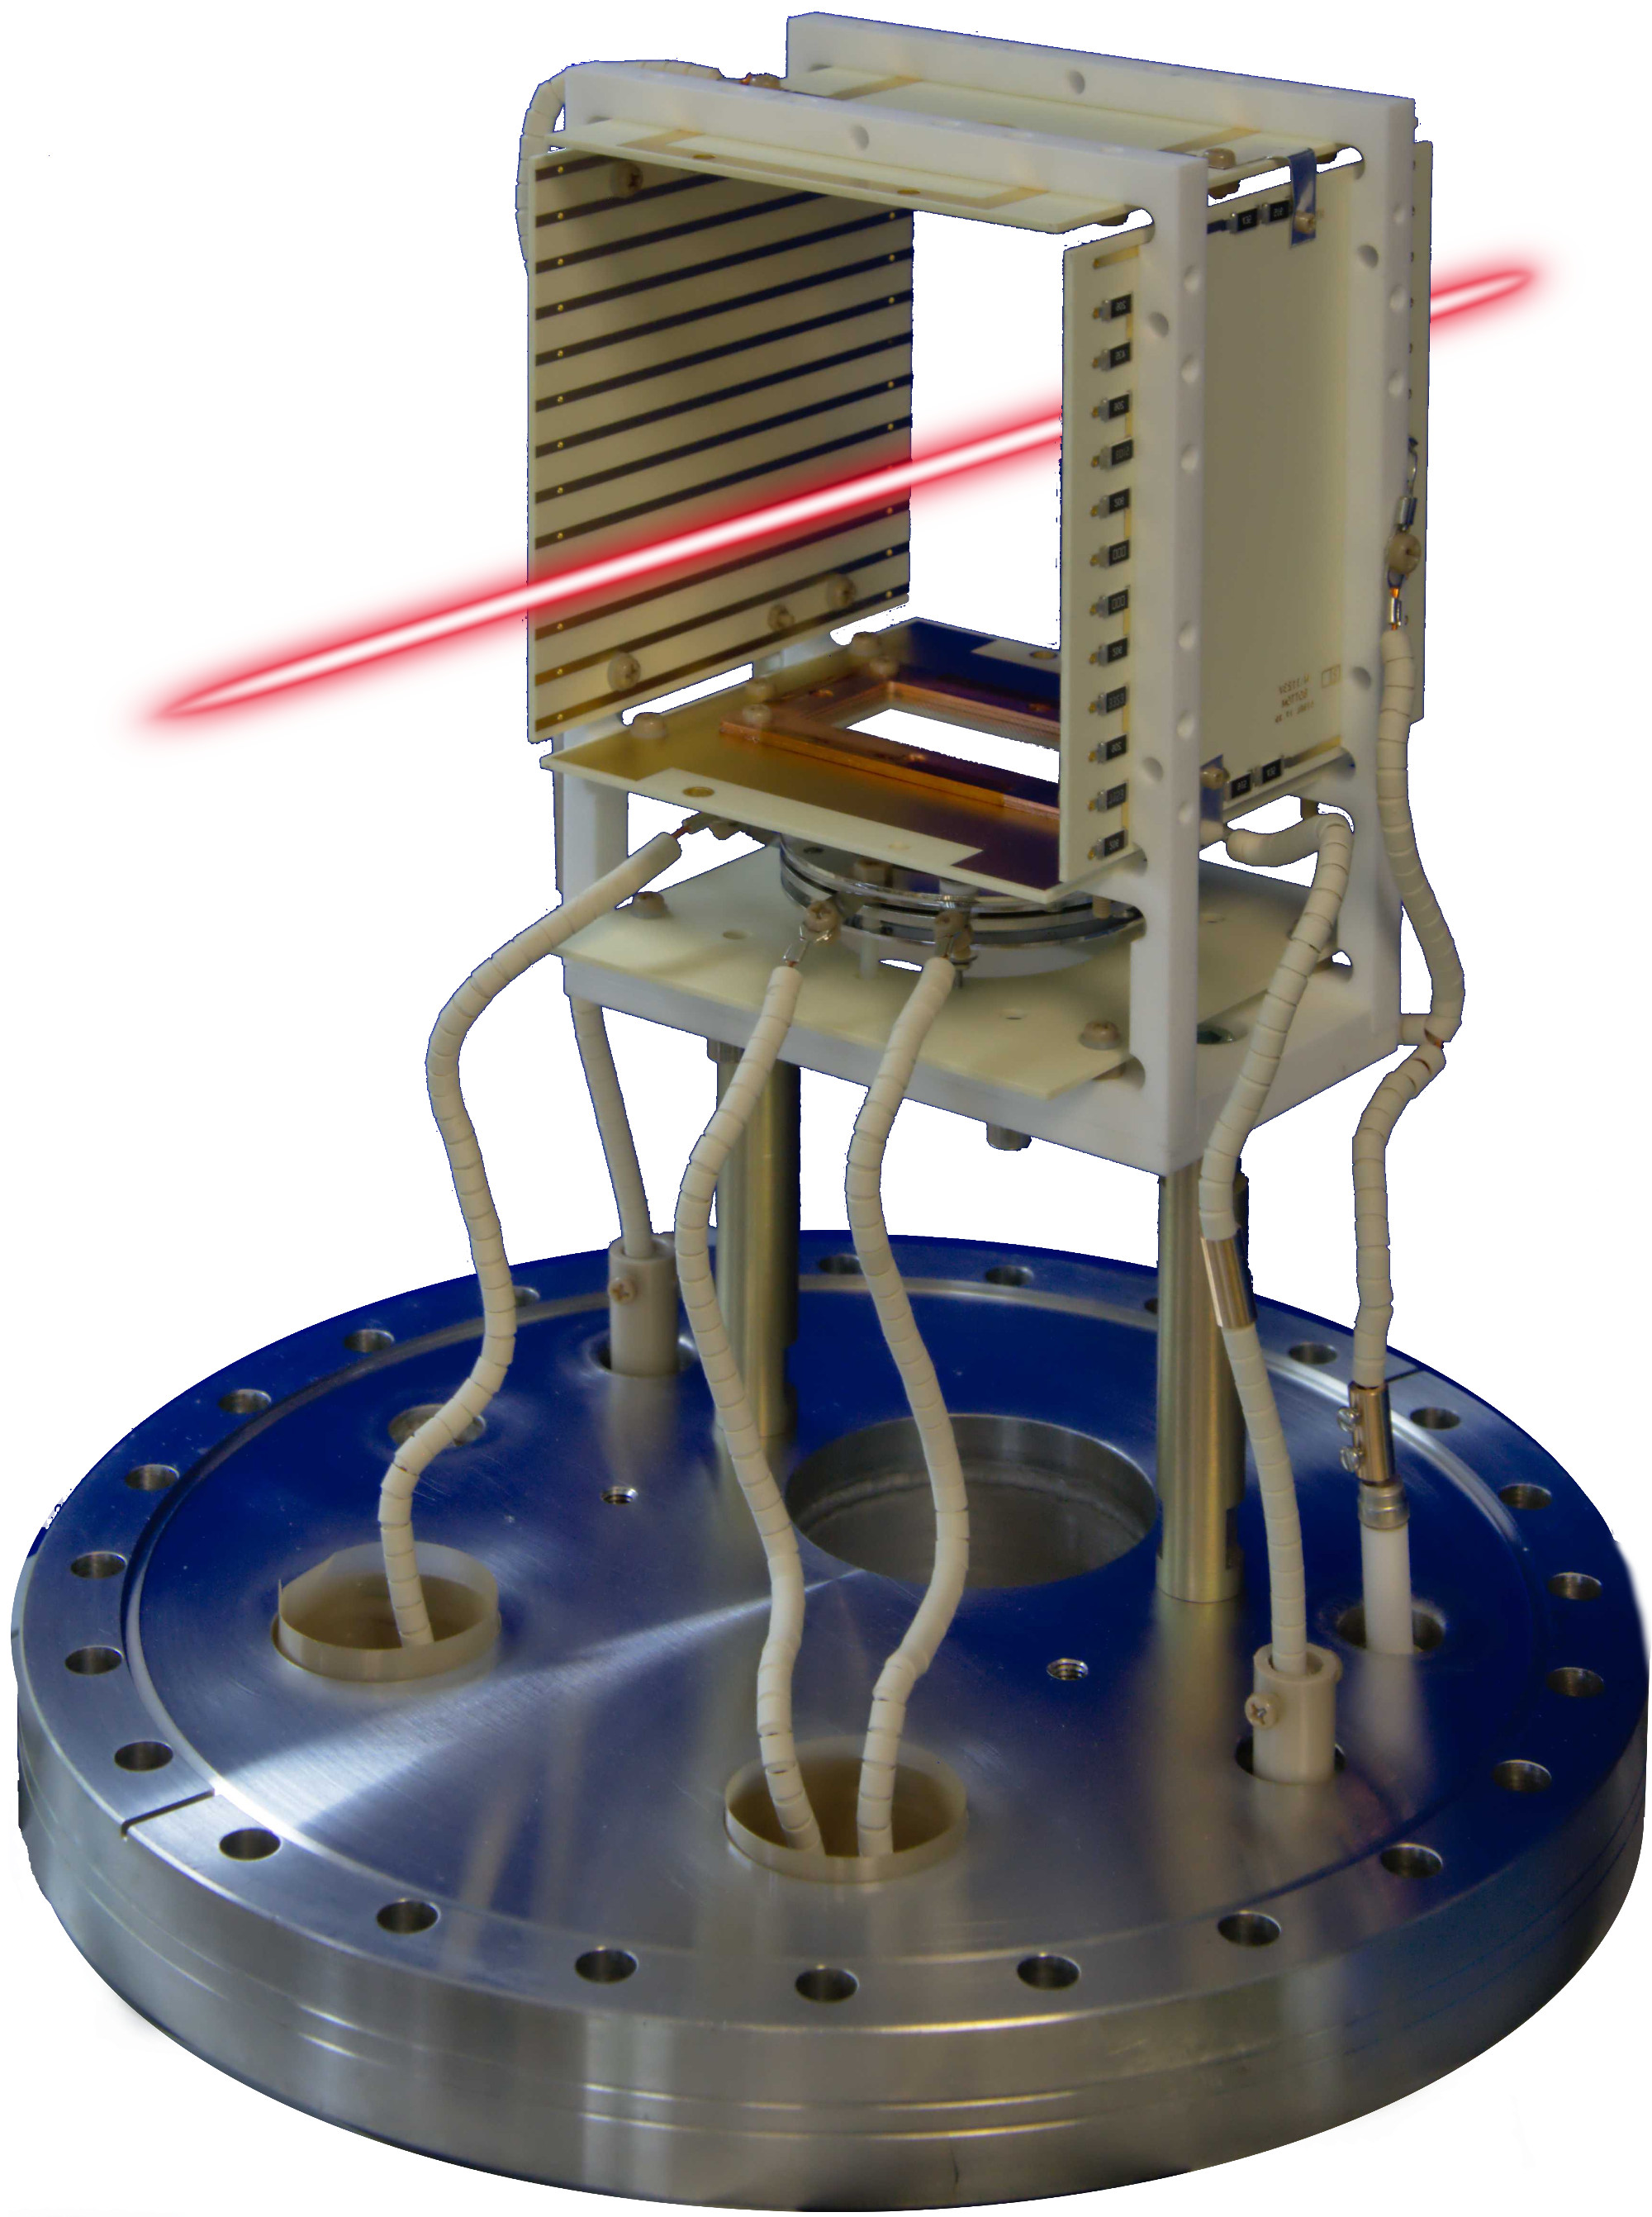
\includegraphics[width=0.35\textwidth]{00_French/figures/fig000_IPM_photo2_fr}
  \caption[]{Photographie d'un des prototypes.}
  \label{chap4:IPM_photo2}
\end{wrapfigure}

Après ces tests préliminaires le travail s'est concentré sur les IPM. Dans les faits nous avons développé plusieurs prototypes et un banc de test permettant de tester ces prototypes. Nous avons également investigué sur des méthodes de référence afin de comparer avec les mesures faites IPMs. L’ensemble des composants a été intégré au fur et à mesure à plusieurs niveaux (mécanique, électronique, informatique), il s’agit plus d’une plateforme de test que d’un simple prototype. Finalement nous avons eu l'occasion de tester nos détecteurs en faisceau à l'accélérateur de proton IPHI. L'énergie de cet accélérateur est plus faible que celle de ESS néanmoins possède de nombreuses caractéristiques identiques. Celles-ci sont données dans la Table \ref{sumfr:tab:IPHI_carac}.

Les deux types d’IPM (plancher conducteur et MCP) ont été testés à IPHI et ont correctement fonctionné durant deux campagnes de tests. La Figure \ref{sumfr:fig:profil} illustre un exemple de profil mesuré par les deux types d’IPM. Une complète caractérisation des détecteurs a été effectuée afin de sélectionner le système de détection le plus adapté aux besoins de ESS.
\begin{table}[!h]
  \centering
  \caption[]{Comparaison entre les accélérateurs IPHI et ESS.}
  \label{sumfr:tab:IPHI_carac}
  \begin{tabularx}{\linewidth}{XXX}
    \toprule
                 & IPHI                                              & ESS                            \\
    \midrule
    Energie      & $3\,\mathrm{MeV}$                                 & $2\,\mathrm{GeV}$              \\
    Courant max. & $100\,\mathrm{mA}$                                & $62.5\,\mathrm{mA}$            \\
    Durée pulse  & up to DC                                          & $2.86\,\mathrm{ms}$            \\
    Répétition   & -                                                 & $14\,\mathrm{Hz}$              \\
    Vide         & $5\cdot10^{-7}$ to $1\cdot10^{-8}\,\mathrm{mbar}$ & $1\cdot10^{-9}\,\mathrm{mbar}$ \\
    \bottomrule
  \end{tabularx}
\end{table}

Les IPM permettent également de mesurer plusieurs informations autres que le profil. Il est possible de comparer ces mesures à celles effectuées par des diagnostics déjà présents à IPHI\footnote{Il n’y pas de diagnostics de profil sur IPHI.}. La Figure \ref{sumfr:fig:beam_car} montre l'excellente relation entre le courant et la position du faisceau mesurés par les IPM et des diagnostics de références présents sur IPHI. Les modèles de simulations développés ont également pu être confortés à l’aide des nombreuses données expérimentales.

\begin{figure}[!ht]
	\begin{subfigure}[t]{0.55\textwidth}
		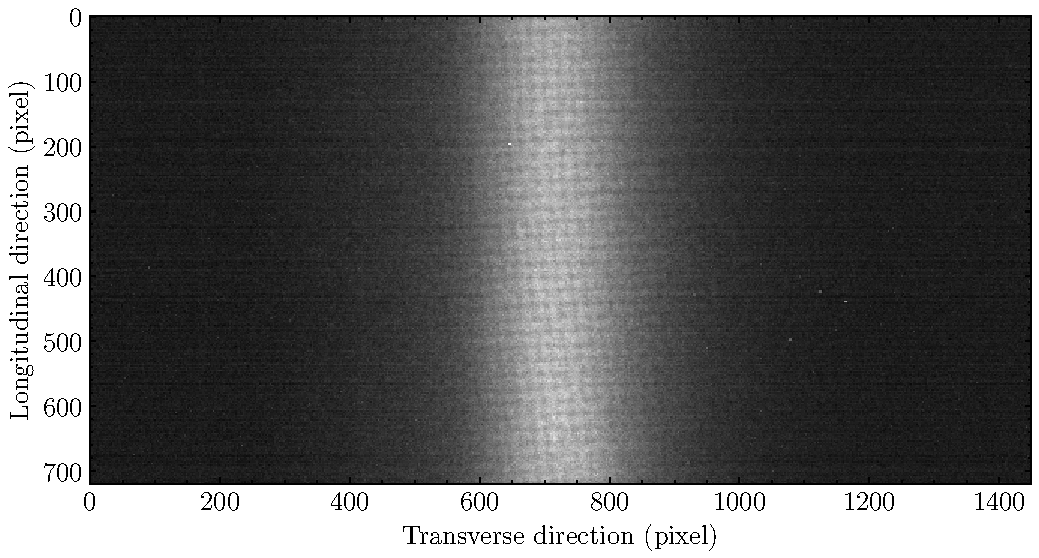
\includegraphics[width=\textwidth]{00_French/figures/fig000_profil_a}
		\caption[]{Image brute provenant d'un IPM avec MCP.}
		\label{sumfr:fig:profil_a}
	\end{subfigure}
	~
	\begin{subfigure}[t]{0.45\textwidth}
		\includesvg[width=\textwidth]{00_French/figures/fig000_profil_b}
		\caption[]{Superposition d'un profil faisceau mesuré avec les deux IPM.}
		\label{sumfr:fig:profil_b}
	\end{subfigure}
  \caption[]{Exemple de mesures de profils avec les deux types d'IPM.}
	\label{sumfr:fig:profil}
\end{figure}

\begin{figure}[!ht]
	\begin{subfigure}[t]{0.5\textwidth}
		\includesvg[width=\textwidth]{00_French/figures/fig000_beam_car_a}
		\caption[]{La position du faisceau enregistrée par un IPM et par un moniteur de position.}
		\label{sumfr:fig:beam_car_a}
	\end{subfigure}
	~
	\begin{subfigure}[t]{0.45\textwidth}
		\includesvg[width=\textwidth]{00_French/figures/fig000_beam_car_b}
		\caption[]{Le signal d'un IPM est proportionnel au courant du faisceau.}
		\label{sumfr:fig:beam_car_b}
	\end{subfigure}
  \caption[]{Les mesures des IPM ont été comparées à des mesures de références.}
	\label{sumfr:fig:beam_car}
\end{figure}


L'un des aspects fondamentaux à vérifier est la possibilité de détecter dans des conditions proches de ESS. En effet, IPHI étant un accélérateur de plus basse énergies le signal est beaucoup plus important. Mais il est possible de réduire la durée et le courant du faisceau pour atteindre des conditions similaires. Ces tests ont été effectués sur les deux types d’IPM. Les résultats montrent que l’utilisation d’un MCP est nécessaire pour mesurer correctement le profil dans des conditions ESS. 

L’ensemble des résultats ont été présentés et approuvé lors d’une Critical Design Review marquant l’entrée du projet dans la phase de production. Actuellement le design final est en train d’être figé avec de nombreuses améliorations qui tenant compte du retour d’expérience. Les premiers tests sont prévus pour la fin 2019 pour assurer une livraison à ESS en début d’année 2020. Dans le même temps, les modèles de simulations sont mis à jour et amélioré pour 

% Perspective
Pour finir sur une perspective différente que le projet ESS. Depuis les trois dernières années, une nouvelle dynamique est en marche pour exploiter pleinement les capacités de IPHI. Aujourd'hui, IPHI est la première étape d'un nouveau projet de source de neutrons compacte nationale : SONATE.
Lors des tests, la versatilité de IPHI a grandement aidé à caractériser les IPM. En retour les IPM ont pu fournir des informations inédites à propos du faisceau. Les IPM sont particulièrement bien adaptés pour un faisceau intense comme IPHI. C'est pourquoi une collaboration étroite a démarré afin de fournir à IPHI un ensemble d'IPM permettant de répondre aux besoins présents et futurs. Ce nouveau projet va grandement bénéficier des études et des expériences présentées dans cette thèse.